%---------------------------------------------------------------------
%
%                          Cap�tulo 5
%
%---------------------------------------------------------------------
%
% 05Bibliografia.tex
% Copyright 2009 Marco Antonio Gomez-Martin, Pedro Pablo Gomez-Martin
%
% This file belongs to the TeXiS manual, a LaTeX template for writting
% Thesis and other documents. The complete last TeXiS package can
% be obtained from http://gaia.fdi.ucm.es/projects/texis/
%
% Although the TeXiS template itself is distributed under the 
% conditions of the LaTeX Project Public License
% (http://www.latex-project.org/lppl.txt), the manual content
% uses the CC-BY-SA license that stays that you are free:
%
%    - to share & to copy, distribute and transmit the work
%    - to remix and to adapt the work
%
% under the following conditions:
%
%    - Attribution: you must attribute the work in the manner
%      specified by the author or licensor (but not in any way that
%      suggests that they endorse you or your use of the work).
%    - Share Alike: if you alter, transform, or build upon this
%      work, you may distribute the resulting work only under the
%      same, similar or a compatible license.
%
% The complete license is available in
% http://creativecommons.org/licenses/by-sa/3.0/legalcode
%
%---------------------------------------------------------------------

\chapter{Pruebas con usuarios}
\label{cap5}
\label{cap:pruebas}


En las fases finales del desarrollo de la herramienta se llev\'o a cabo otro desarrollo en paralelo. Este desarrollo era la implementaci\'on de la herramienta desarrollada en un juego ya terminado y cerrado para realizar pruebas de rendimiento y usabilidad con usuarios. Los usuarios seleccionados no hab\'ian tenido contacto previo con la herramienta ni con el juego elegido. En este cap\'itulo se recogen los objetivos
de las pruebas, se analizar\'an los resultados obtenidos y se sacar\'an conclusiones al respecto.

%-------------------------------------------------------------------
\section{Realizaci\'on de Demo}
%-------------------------------------------------------------------

Durante las fases finales de la implementaci\'on de la herramienta se vio la necesidad de integrar esta herramienta en un proyecto ya terminado en el que poder realizar pruebas de rendimiento, comprobar si era necesaria la implementaci\'on de m\'as m\'odulos que los descritos en la especificaci\'on de a herramienta y probarlo en diferentes configuraciones. Para poder realizar estas pruebas era necesario desarrollar un proyecto en paralelo donde poder probar o buscar uno ya terminado. Tras hacer una b\'usqueda de proyectos que pudieran aprovechar la herramienta se propuso la utilizaci\'on de uno de los proyectos que ofrece Unity en su plataforma de aprendizaje \textbf{\textit{Unity Learn}}.\footnote{Unity Learn - https://learn.unity.com/projects} En esta plataforma se encuentran varios proyectos en los cuales pueden incluirse diferentes modificaciones explicadas en la propia plataforma para aprender a utilizar algunos aspectos de Unity. El proyecto escogido de la plataforma ha sido \textbf{Karting Microgame}\footnote{Enlace de descarga en Asset Store - https://assetstore.unity.com/packages/templates/karting-microgame-150956?}, un juego de conducci\'on arcade muy parecido a la saga de \textbf{\textit{Mario Kart}} desarrollada por Nintendo. Se escogi\'o este juego por su similitud a una saga qla cual ha jugado una gran cantidad de poblaci\'on en alg\'un momento ya que cuenta con 17 juegos para una gran variedad de plataformas (iPhone, Android, Nintendo Switch, Wii U, Nintendo 3DS, Wii, Nintendo DS, GameCube, Game Boy Advance y Nintendo 64).

Una vez se han incluido en el proyecto los scripts pertenecientes a la herramienta, se necesitaba una forma de conectar el dispositivo m\'ovil al juego y para esto se implement\'o en la demo de Unity un generador de c\'odigos QR utilizando la libreria \textbf{ZXingNet}\footnote{ZXingNet - https://archive.codeplex.com/?p=zxingnet}. Esta librer\'ia es un port del proyecto ZXing desarrollado en java para leer y generar c\'odigos de barras. Con este c\'odigo QR se env\'ia a la aplicaci\'on m\'ovil los datos de IP y puerto al que debe conectarse para poder ser usado como mando. 

En el proyecto de Unity se debe a\~nadir una nueva c\'amara para poder enviar a la aplicaci\'on Android la imagen del mando. Junto con esta imagen debe incluirse un nuevo script que defina la posici\'on, el alto y el ancho del bot\'on y la acci\'on que se debe realizar cuando el jugador lo pulse. Con esto, cuando las pulsaciones del usuario lleguen al juego podr\'an ser tratadas como si fuesen teclas. 

Para hacer el juego juegable tanto con el nuevo input como con el original, se ha a\~nadido un peque\~no men\'u al inicio del juego para elegir qu\'e input utilizar. Para poder salir del juego de manera controlada tambi\'en se ha a\~nadido un bot\'on para poder salir de la aplicaci\'on.

Para leer este QR desde la aplicaci\'on m\'ovil se ha a\~nadido una Activdad nueva que se ejecuta al inicio de la aplicaci\'on. Esta Actividad tiene como funci\'on utilizar la c\'amara del dispositivo Android para leer el QR y guardarse esos datos. Estos datos se mandan a la siguiente Actividad donde la aplicaci\'on los utilizar\'a para iniciar la conexi\'on y poder ser utilizada como dispositivo de entrada.

\begin{figure}[!htb]
\begin{minipage}{0.5\textwidth}
\centering
\includegraphics[width=0.8\textwidth]{./Imagenes/Bitmap/Menu_Principal_Juego}
\caption{Inicio Demo Unity}
\end{minipage}\hfill
\begin{minipage}{0.6\textwidth}
\centering
\includegraphics[width=1.0\textwidth]{./Imagenes/Bitmap/Mando}
\caption{Mando Demo Android}
\end{minipage}
\end{figure}

%-------------------------------------------------------------------
\section{Objetivos y organizaci\'on de las pruebas}
%-------------------------------------------------------------------

Previo a las pruebas con usuarios se definieron una serie de objetivos que cubrir durante la evaluaci\'on. Estos objetivos son los siguientes:

\begin {itemize}
\item Comprobaci\'on del funcionamiento de ambas aplicaciones (Android y Unity) en diferentes configuraciones.
\item Rendimiento de la parte de red, sobretodo en el env\'io de im\'agenes y el tiempo de env\'io de las pulsaciones.
\item Valorar la intuitividad del uso de la herramienta.
\end {itemize}

Debido a la pandemia mundial que tuvo lugar durante la publicaci\'on de esta memoria debido al confinamiento por el virus SARS-COV-2, tambi\'en conocido como \textit{Coronavirus}, las pruebas de usuario han tenido que modificarse y adaptarse para ser realizadas de manera online en lugar de f\'isicamente. Todas las pruebas se han realizado siguiendo las siguientes pautas:

\begin {itemize}
\item Se ha informado al usuario de los datos t\'ecnicos que se van a extraer de esta prueba (modelo de tarjeta gr\'afica, modelo de procesador, memoria RAM) y del posterior formulario a rellenar.
\item Se ha subido el ejecutable y el APK a un repositorio p\'ublico para que el usuario pueda hacer las pruebas.
\item Se ha indicado al usuario que el ordenador y el m\'ovil deben estar conectados a la misma red WIFI.
\item Se ha utilizado la aplicaci\'on de \textbf{Discord} para realizar una llamada con el usuario y que este compartiese la pantalla donde se estaba ejecutando el juego.
\item Se ha explicado al jugador que tiene que escanear el c\'odigo QR que aparece en el juego con la aplicaci\'on que se ha descargado del repositorio.
\item Se ha indicado al usuario que debe dar varias vueltas al circuito para que los datos puedan recogerse. 
\item Se ha realizado una entrevista con el usuario de entre 5 y 10 minutos para rellenar el formulario y comentar cualquier tipo de \textit{feedback} sobre la herramienta y el juego.
\end {itemize}

Al final de la prueba se realiza una charla con el usuario donde este nos indica todas las observaciones, sugerencias de mejora y puntos positivos. En esta charla tambi\'en se hacen algunas preguntas como por ejemplo el modelo de m\'ovil con el que ha realizado la prueba, experiencia jugando a videojuegos y cuales juega normalmente, opini\'on sobre la fluidez de la prueba y el \textit{feedback} recibido (visual y h\'aptico gracias a la vibraci\'on).

%-------------------------------------------------------------------
\section{Resultados de las pruebas}
%-------------------------------------------------------------------

En total, este experimento ha contado con 5 participantes que se han ofrecido voluntariamente a probar la herramienta. A pesar de contar con un n\'umero muy limitado de usuarios se han obtenido opiniones variadas. Entre los usuarios se encuentran tanto jugadores habituales de videojuegos como usuarios que no juegan. Los resultados individuales de las pruebas son:

\begin{enumerate}
  \item \textbf{Usuario 1}

Este usuario tiene 22 a\~nos y es un jugador habitual. Suele jugar en PC a juegos como World of Warcraft, Crossfire, Monster Hunter y Starcraft 2.
Las pruebas se han realizado con los siguientes dispositivos: \\

\begin{tabularx}{1.0\textwidth} { 
  | >{\centering\arraybackslash}X 
  | >{\centering\arraybackslash}X 
  | >{\centering\arraybackslash}X 
  | >{\centering\arraybackslash}X | }
 \hline
 \textbf{Tarjeta Gr\'afica} & \textbf{Procesador} & \textbf{RAM} & \textbf{Modelo M\'ovil} \\
 \hline
 NVIDIA GeForce GTX 980  & Intel(R) Core(TM) i7-5820K CPU @ 3.30GHz  & 32594 MB & One plus 6  \\
\hline
\end{tabularx}
\\
Se han recogido los diferentes tiempos que tarda Unity en convertir la imagen que se optiene de la c\'amara a formato PNG, enviarse por red al dispositivo Android y el tiempo que este tarda en descomprimir el PNG y mostrar la imagen en la pantalla. 

Este usuario coment\'o durante la prueba que la vibraci\'on era adecuada a la hora de pulsar los botones. Se\~nal\'o tambi\'en que los botones le parecian muy peque\~nos y que necesitar\'ian ser m\'as grandes ya que hay veces que no se pulsan bien. En cuanto a si la experiencia fue fluida, el usuario contest\'o un 7 sobre 8 siendo 1 - Nada fluida y 8 - Completamente fluida. Cabe destacar que la latencia de red en el momento de la prueba era de 2 milisegundos.

\begin{figure}[!h]
\centering
\resizebox{0.5\textwidth}{!}{%
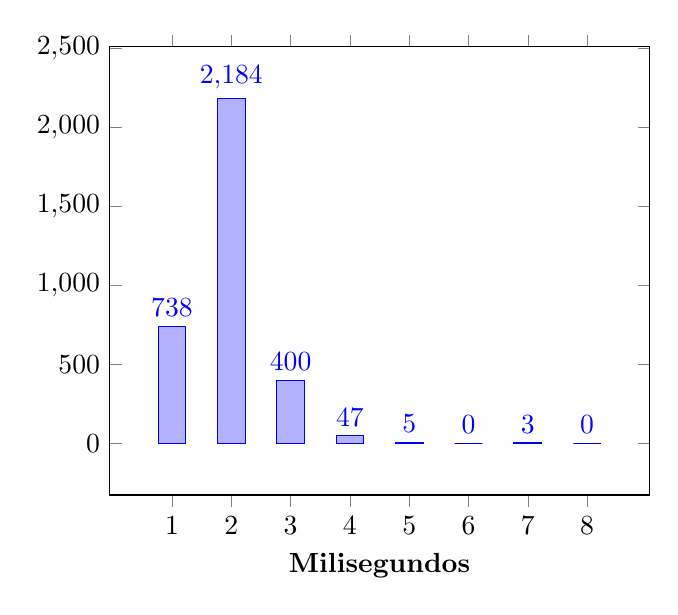
\begin{tikzpicture}
\begin{axis}[
    ybar,
    enlargelimits=0.15,
    legend style={at={(0.5,-0.15)},
    anchor=north,legend columns=-1},
    xlabel={\textbf{Milisegundos}},
    symbolic x coords={1,2,3,4,5,6,7,8},
    xtick=data,
    nodes near coords,
    nodes near coords align={vertical},
    ]
\addplot coordinates {(1,738) (2,2184) (3,400) (4,47) (5,5) (6,0) (7,3) (8,0)};
\end{axis}
\end{tikzpicture}
}%
\caption{Tiempo de descompresi\'on PNG en dispositivo Android Usuario 1}
\end{figure}

\begin{figure}[!h]
\centering
\resizebox{0.5\textwidth}{!}{%
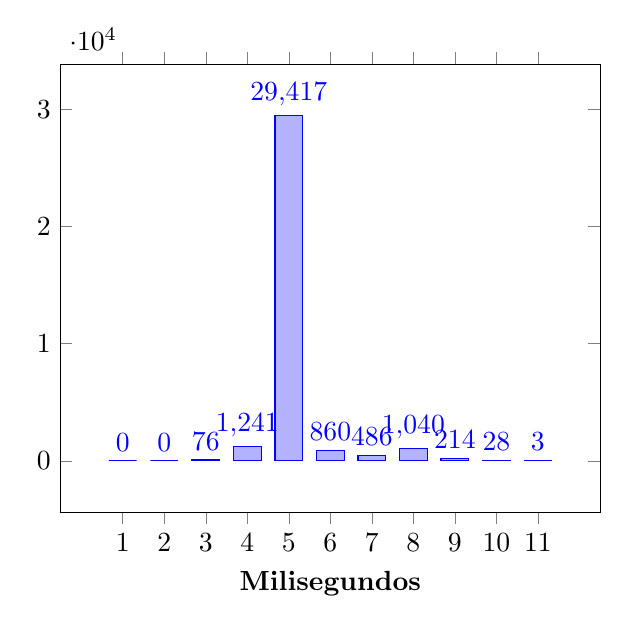
\begin{tikzpicture}
\begin{axis}[
    ybar,
    enlargelimits=0.15,
    legend style={at={(0.5,-0.15)},
    anchor=north,legend columns=-1},
    xlabel={\textbf{Milisegundos}},
    symbolic x coords={1,2,3,4,5,6,7,8,9,10,11},
    xtick=data,
    nodes near coords,
    nodes near coords align={vertical},
    ]
\addplot coordinates {(1,0) (2,0) (3,76) (4,1241) (5,29417) (6,860) (7,486) (8,1040) (9,214) (10,28) (11,3)};
\end{axis}
\end{tikzpicture}
}%
\caption{Tiempo de conversi\'on de c\'arama de Unity a PNG Usuario 1}
\end{figure}

Con los dispositivos utilizados se obtiene una media en milisegundos de descompresi\'on de PNG de XX y de transformaci\'on de textura de Unity a PNG de XX. La moda en la descompresi\'on del PNG es de 2 milisegundos y la moda en el tiempo de conversi\'on de textura a PNG es de 5 milisegundos. Sumado a esto tenemos los 2 milisegundos de latencia por lo que el proceso completo estar\'ia en los 9 milisegundos en la mayor\'ia de los casos. El umbral en el que el ojo humano detecta un cambio en las im\'agenes es de 14 milisegundos por lo que al encontrarse por debajo podemos asegurar que la fluidez durante la sesi\'on fue la \'optima.
%---------------------------------------------------------------------
%---------------------------------------------------------------------
%---------------------------------------------------------------------
%---------------------------------------------------------------------

\newpage \item \textbf{Usuario 2}

Este usuario tiene 23 a\~nos y es un jugador habitual. Suele jugar a juegos como Call Of Duty: MW, Dragalia Lost y Mario Kart 8.
Las pruebas se han realizado con los siguientes dispositivos: \\

\begin{tabularx}{1.0\textwidth} { 
  | >{\centering\arraybackslash}X 
  | >{\centering\arraybackslash}X 
  | >{\centering\arraybackslash}X 
  | >{\centering\arraybackslash}X | }
 \hline
 \textbf{Tarjeta Gr\'afica} & \textbf{Procesador} & \textbf{RAM} & \textbf{Modelo M\'ovil} \\
 \hline
 NVIDIA GeForce GTX 1080  &Intel(R) Core(TM) i7-6700K CPU @ 4.00GHz  & 16327 MB & One plus 6  \\
\hline
\end{tabularx}


Se han recogido los diferentes tiempos que tarda Unity en convertir la imagen que se optiene de la c\'amara a formato PNG, enviarse por red al dispositivo Android y el tiempo que este tarda en descomprimir el PNG y mostrar la imagen en la pantalla. 

Este usuario coment\'o durante la prueba que la vibraci\'on durante los derrapes era intermitente en vez de mantenida. Esto le desagrad\'o. En cuanto a si la experiencia fue fluida, el usuario contest\'o un 8 sobre 8 siendo 1 - Nada fluida y 8 - Completamente fluida. Cabe destacar que la latencia de red en el momento de la prueba era de 3 milisegundos.

\begin{figure}[!h]
\centering
\resizebox{0.5\textwidth}{!}{%
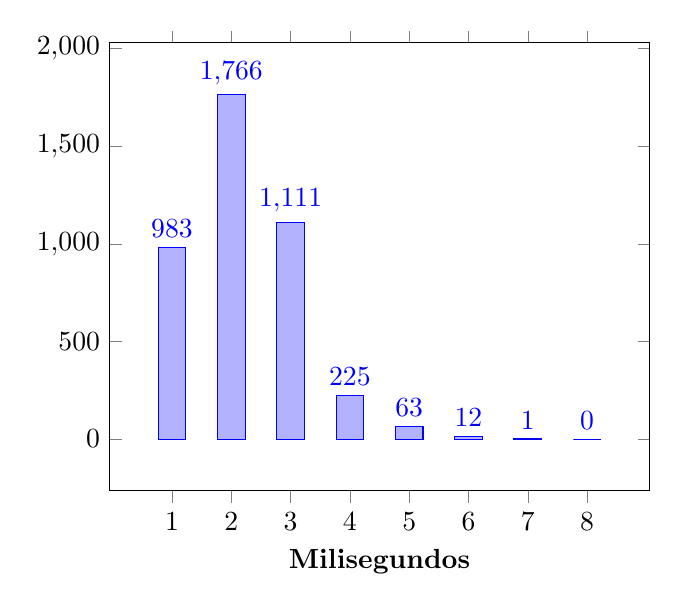
\begin{tikzpicture}
\begin{axis}[
    ybar,
    enlargelimits=0.15,
    legend style={at={(0.5,-0.15)},
    anchor=north,legend columns=-1},
    xlabel={\textbf{Milisegundos}},
    symbolic x coords={1,2,3,4,5,6,7,8},
    xtick=data,
    nodes near coords,
    nodes near coords align={vertical},
    ]
\addplot coordinates {(1,983) (2,1766) (3,1111) (4,225) (5,63) (6,12) (7,1) (8,0)};
\end{axis}
\end{tikzpicture}
}%
\caption{Tiempo de descompresi\'on PNG en dispositivo Android Usuario 2}
\end{figure}

\begin{figure}[!h]
\centering
\resizebox{0.5\textwidth}{!}{%
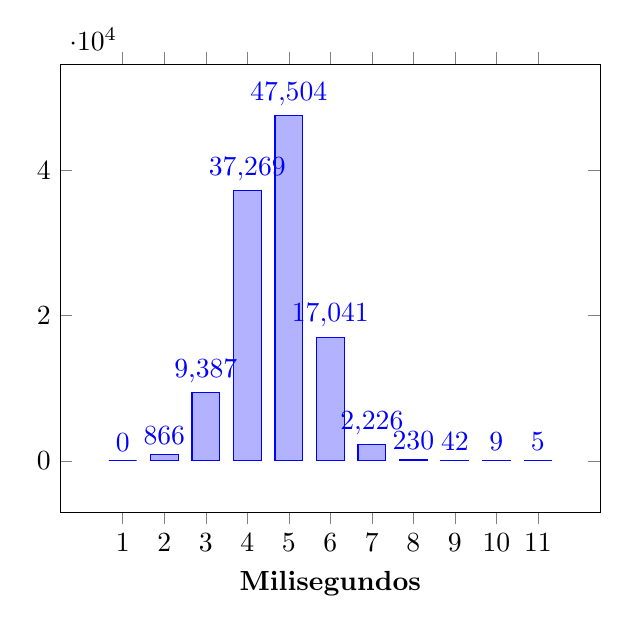
\begin{tikzpicture}
\begin{axis}[
    ybar,
    enlargelimits=0.15,
    legend style={at={(0.5,-0.15)},
    anchor=north,legend columns=-1},
    xlabel={\textbf{Milisegundos}},
    symbolic x coords={1,2,3,4,5,6,7,8,9,10,11},
    xtick=data,
    nodes near coords,
    nodes near coords align={vertical},
    ]
\addplot coordinates {(1,0) (2,866) (3,9387) (4,37269) (5,47504) (6,17041) (7,2226) (8,230) (9,42) (10,9) (11,5)};
\end{axis}
\end{tikzpicture}
}%
\caption{Tiempo de conversi\'on de c\'arama de Unity a PNG Usuario 2}
\end{figure}

Con los dispositivos utilizados se obtiene una media en milisegundos de descompresi\'on de PNG de XX y de transformaci\'on de textura de Unity a PNG de XX. La moda en la descompresi\'on del PNG es de 2-3 milisegundos y la moda en el tiempo de conversi\'on de textura a PNG es de 4 y 5 milisegundos la mayor parte de las veces. Sumado a esto tenemos los 3 milisegundos de latencia por lo que el proceso completo estar\'ia entre 9-11 milisegundos en la mayor\'ia de los casos. El umbral en el que el ojo humano detecta un cambio en las im\'agenes es de 14 milisegundos por lo que al encontrarse por debajo podemos asegurar que la fluidez durante la sesi\'on fue la \'optima.

%---------------------------------------------------------------------
%---------------------------------------------------------------------
%---------------------------------------------------------------------
%---------------------------------------------------------------------
\item \textbf{Usuario 3}

Este usuario tiene 49 a\~nos y es un jugador casual. Suele jugar a juegos como Age of Empires, Destiny, ARK y La Batalla por la Tierra Miedia.
Las pruebas se han realizado con los siguientes dispositivos: \\

\begin{tabularx}{1.0\textwidth} { 
  | >{\centering\arraybackslash}X 
  | >{\centering\arraybackslash}X 
  | >{\centering\arraybackslash}X 
  | >{\centering\arraybackslash}X | }
 \hline
 \textbf{Tarjeta Gr\'afica} & \textbf{Procesador} & \textbf{RAM} & \textbf{Modelo M\'ovil} \\
 \hline
 NVIDIA GeForce GTX 960M  & Intel(R) Core(TM) i7-6700HQ CPU @ 2.60GHz  & 16289 MB & Samsung Galaxy S9+  \\
\hline
\end{tabularx}


Se han recogido los diferentes tiempos que tarda Unity en convertir la imagen que se optiene de la c\'amara a formato PNG, enviarse por red al dispositivo Android y el tiempo que este tarda en descomprimir el PNG y mostrar la imagen en la pantalla. 

Este usuario coment\'o durante la prueba que la vibraci\'on era demasiado fuerte por lo que deber\'ia de disminuir la intensidad. Esto le desagrad\'o. En cuanto a si la experiencia fue fluida, el usuario contest\'o un 5 sobre 8 siendo 1 - Nada fluida y 8 - Completamente fluida. Cabe destacar que la latencia de red en el momento de la prueba era de 2 milisegundos.

\begin{figure}[!h]
\centering
\resizebox{0.5\textwidth}{!}{%
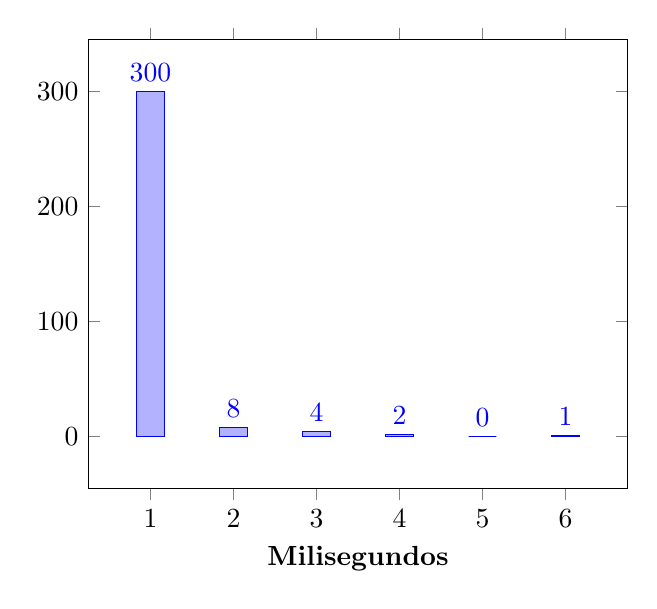
\begin{tikzpicture}
\begin{axis}[
    ybar,
    enlargelimits=0.15,
    legend style={at={(0.5,-0.15)},
    anchor=north,legend columns=-1},
    xlabel={\textbf{Milisegundos}},
    symbolic x coords={1,2,3,4,5,6},
    xtick=data,
    nodes near coords,
    nodes near coords align={vertical},
    ]
\addplot coordinates {(1,300) (2,8) (3,4) (4,2) (5,0) (6,1)};
\end{axis}
\end{tikzpicture}
}%
\caption{Tiempo de descompresi\'on PNG en dispositivo Android Usuario 3}
\end{figure}

\begin{figure}[!h]
\centering
\resizebox{0.5\textwidth}{!}{%
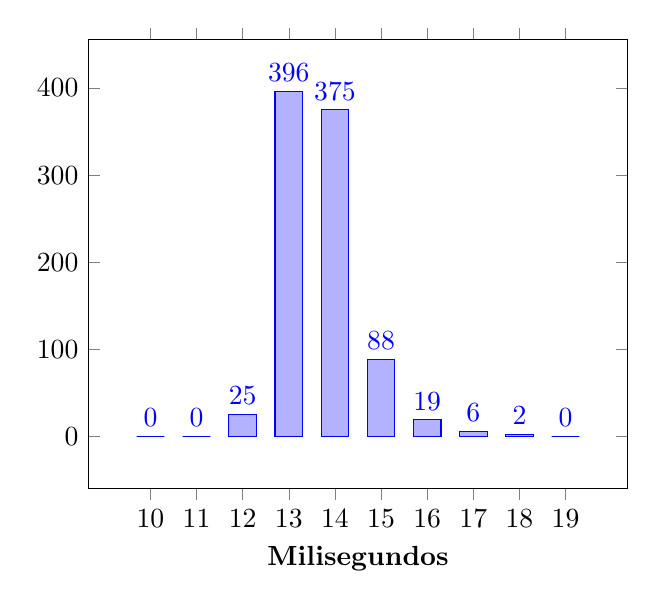
\begin{tikzpicture}
\begin{axis}[
    ybar,
    enlargelimits=0.15,
    legend style={at={(0.5,-0.15)},
    anchor=north,legend columns=-1},
    xlabel={\textbf{Milisegundos}},
    symbolic x coords={10,11,12,13,14,15,16,17,18,19},
    xtick=data,
    nodes near coords,
    nodes near coords align={vertical},
    ]
\addplot coordinates {(10,0) (11,0) (12,25) (13,396) (14,375) (15,88) (16,19) (17,6) (18,2) (19,0)};
\end{axis}
\end{tikzpicture}
}%
\caption{Tiempo de conversi\'on de c\'arama de Unity a PNG Usuario 3}
\end{figure}

Con los dispositivos utilizados se obtiene una media en milisegundos de descompresi\'on de PNG de XX y de transformaci\'on de textura de Unity a PNG de XX. La moda en la descompresi\'on del PNG es de 1 milisegundos y la moda en el tiempo de conversi\'on de textura a PNG es de 13 y 14 milisegundos la mayor parte de las veces. Sumado a esto tenemos los 2 milisegundos de latencia por lo que el proceso completo estar\'ia entre 16 y 17 milisegundos en la mayor\'ia de los casos. El umbral en el que el ojo humano detecta un cambio en las im\'agenes es de 14 milisegundos por lo que al encontrarse por encima la fluidez no ha sido la \'optima.

%---------------------------------------------------------------------
%---------------------------------------------------------------------
%---------------------------------------------------------------------
%---------------------------------------------------------------------

\item \textbf{Usuario 4}

Este usuario tiene 51 a\~nos y no juega a videojuegos salvo en momentos muy concretos. Los juegos a los que ha jugado en alg\'un momento han sido Mario Kart de Wii y Scrabble para Android.
Las pruebas se han realizado con los siguientes dispositivos: \\

\begin{tabularx}{1.0\textwidth} { 
  | >{\centering\arraybackslash}X 
  | >{\centering\arraybackslash}X 
  | >{\centering\arraybackslash}X 
  | >{\centering\arraybackslash}X | }
 \hline
 \textbf{Tarjeta Gr\'afica} & \textbf{Procesador} & \textbf{RAM} & \textbf{Modelo M\'ovil} \\
 \hline
AMD Radeon HD 7660D  & AMD A10-5800K APU with Radeon(tm) HD Graphics  & 7367 MB & Samsung Galaxy S8  \\
\hline
\end{tabularx}


Se han recogido los diferentes tiempos que tarda Unity en convertir la imagen que se optiene de la c\'amara a formato PNG, enviarse por red al dispositivo Android y el tiempo que este tarda en descomprimir el PNG y mostrar la imagen en la pantalla. 

Este usuario coment\'o durante la prueba que los botones no se correspond\'ian por completo con los mostrados en la imagen, ten\'ia que pulsar un poco fuera del bot\'on para que este se detectase. En cuanto a si la experiencia fue fluida, el usuario contest\'o un 7 sobre 8 siendo 1 - Nada fluida y 8 - Completamente fluida. Cabe destacar que la latencia de red en el momento de la prueba era de 2 milisegundos.

\begin{figure}[!h]
\centering
\resizebox{0.5\textwidth}{!}{%
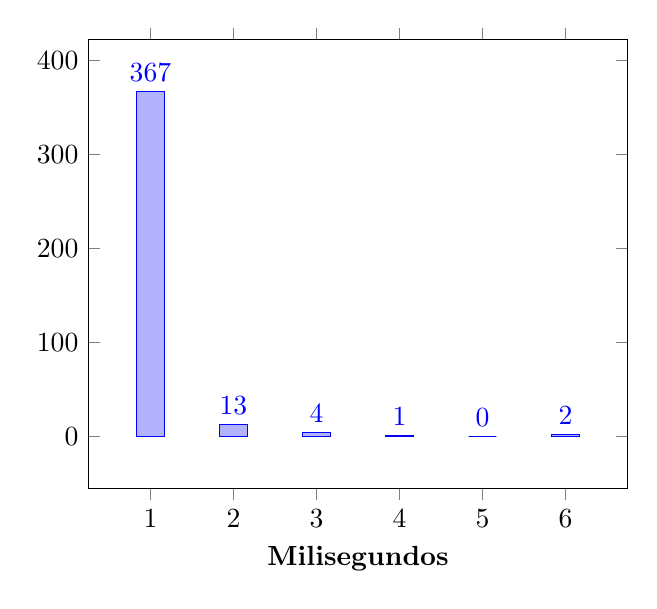
\begin{tikzpicture}
\begin{axis}[
    ybar,
    enlargelimits=0.15,
    legend style={at={(0.5,-0.15)},
    anchor=north,legend columns=-1},
    xlabel={\textbf{Milisegundos}},
    symbolic x coords={1,2,3,4,5,6},
    xtick=data,
    nodes near coords,
    nodes near coords align={vertical},
    ]
\addplot coordinates {(1,367) (2,13) (3,4) (4,1) (5,0) (6,2)};
\end{axis}
\end{tikzpicture}
}%
\caption{Tiempo de descompresi\'on PNG en dispositivo Android Usuario 4}
\end{figure}

\begin{figure}[!h]
\centering
\resizebox{0.5\textwidth}{!}{%
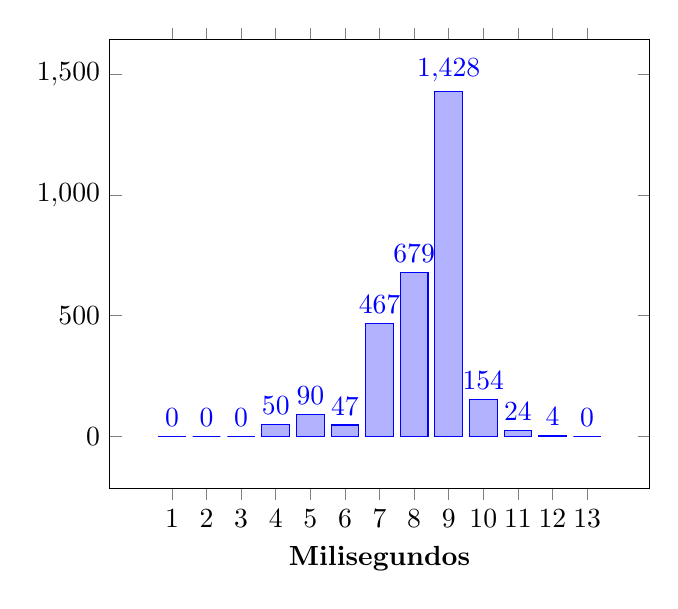
\begin{tikzpicture}
\begin{axis}[
    ybar,
    enlargelimits=0.15,
    legend style={at={(0.5,-0.15)},
    anchor=north,legend columns=-1},
    xlabel={\textbf{Milisegundos}},
    symbolic x coords={1,2,3,4,5,6,7,8,9,10,11,12,13},
    xtick=data,
    nodes near coords,
    nodes near coords align={vertical},
    ]
\addplot coordinates  {(1,0) (2,0) (3,0) (4,50) (5,90) (6,47) (7,467) (8,679) (9,1428) (10,154) (11,24) (12,4) (13,0) };
\end{axis}
\end{tikzpicture}
}%
\caption{Tiempo de conversi\'on de c\'arama de Unity a PNG Usuario 4}
\end{figure}

Con los dispositivos utilizados se obtiene una media en milisegundos de descompresi\'on de PNG de XX y de transformaci\'on de textura de Unity a PNG de XX. La moda en la descompresi\'on del PNG es de 1 milisegundos y la moda en el tiempo de conversi\'on de textura a PNG es de 7-9 milisegundos la mayor parte de las veces. Sumado a esto tenemos los 2 milisegundos de latencia por lo que el proceso completo estar\'ia entre 10-12 milisegundos en la mayor\'ia de los casos. El umbral en el que el ojo humano detecta un cambio en las im\'agenes es de 14 milisegundos por lo que al encontrarse por debajo podemos asegurar que la fluidez durante la sesi\'on fue la \'optima.

%---------------------------------------------------------------------
%---------------------------------------------------------------------
%---------------------------------------------------------------------
%---------------------------------------------------------------------

\item \textbf{Usuario 5}

Este usuario tiene 19 a\~nos y es un jugador habitual de juegos en todas las plataformas actuales (PC, PS4, Switch y Android). Los juegos a los que suele jugar son World Of Warcraft, The Legend of Zelda, Mario Kart, Total War y Assassin's Creed.
Las pruebas se han realizado con los siguientes dispositivos: \\

\begin{tabularx}{1.0\textwidth} { 
  | >{\centering\arraybackslash}X 
  | >{\centering\arraybackslash}X 
  | >{\centering\arraybackslash}X 
  | >{\centering\arraybackslash}X | }
 \hline
 \textbf{Tarjeta Gr\'afica} & \textbf{Procesador} & \textbf{RAM} & \textbf{Modelo M\'ovil} \\
 \hline
NVIDIA GeForce GTX 1080  & Intel(R) Core(TM) i7-6800K CPU @ 3.40GHz  & 32668 MB & Samsung Galaxy S9+  \\
\hline
\end{tabularx}


Se han recogido los diferentes tiempos que tarda Unity en convertir la imagen que se optiene de la c\'amara a formato PNG, enviarse por red al dispositivo Android y el tiempo que este tarda en descomprimir el PNG y mostrar la imagen en la pantalla. 

Este usuario coment\'o durante la prueba que los botones no se correspond\'ian por completo con los mostrados en la imagen, ten\'ia que pulsar un poco fuera del bot\'on para que este se detectase. En cuanto a si la experiencia fue fluida, el usuario contest\'o un 7 sobre 8 siendo 1 - Nada fluida y 8 - Completamente fluida. Cabe destacar que la latencia de red en el momento de la prueba era de 1 milisegundos.

\begin{figure}[!h]
\centering
\resizebox{0.5\textwidth}{!}{%
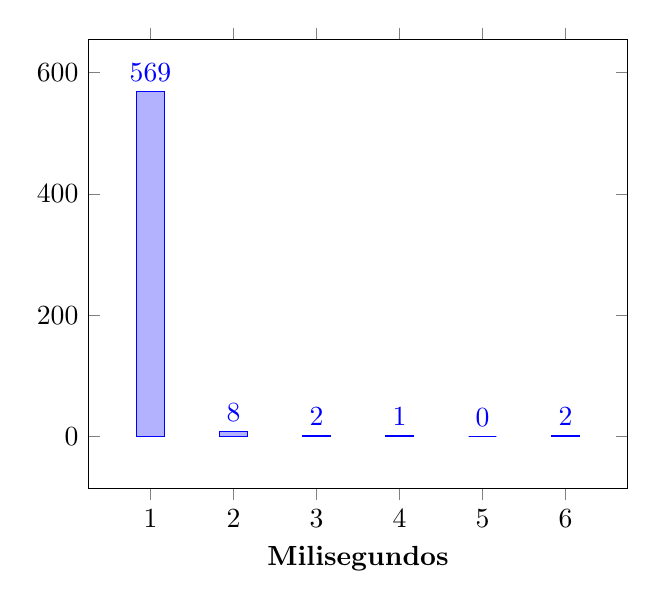
\begin{tikzpicture}
\begin{axis}[
    ybar,
    enlargelimits=0.15,
    legend style={at={(0.5,-0.15)},
    anchor=north,legend columns=-1},
    xlabel={\textbf{Milisegundos}},
    symbolic x coords={1,2,3,4,5,6},
    xtick=data,
    nodes near coords,
    nodes near coords align={vertical},
    ]
\addplot coordinates {(1,569) (2,8) (3,2) (4,1) (5,0) (6,2)};
\end{axis}
\end{tikzpicture}
}%
\caption{Tiempo de descompresi\'on PNG en dispositivo Android Usuario 5}
\end{figure}

\begin{figure}[!h]
\centering
\resizebox{0.5\textwidth}{!}{%
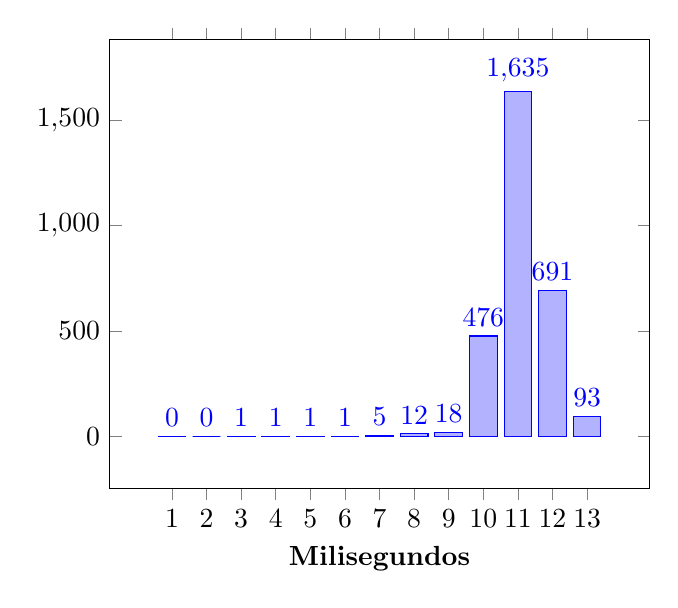
\begin{tikzpicture}
\begin{axis}[
    ybar,
    enlargelimits=0.15,
    legend style={at={(0.5,-0.15)},
    anchor=north,legend columns=-1},
    xlabel={\textbf{Milisegundos}},
    symbolic x coords={1,2,3,4,5,6,7,8,9,10,11,12,13,14,15,16},
    xtick=data,
    nodes near coords,
    nodes near coords align={vertical},
    ]
\addplot coordinates  {(1,0) (2,0) (3,1) (4,1) (5,1) (6,1) (7,5) (8,12) (9,18) (10,476) (11,1635) (12,691) (13,93) };
\end{axis}
\end{tikzpicture}
}%
\caption{Tiempo de conversi\'on de c\'arama de Unity a PNG Usuario 5}
\end{figure}

Con los dispositivos utilizados se obtiene una media en milisegundos de descompresi\'on de PNG de XX y de transformaci\'on de textura de Unity a PNG de XX. La moda en la descompresi\'on del PNG es de 1 milisegundos y la moda en el tiempo de conversi\'on de textura a PNG es de 10-12 milisegundos la mayor parte de las veces. Sumado a esto tenemos los 1 milisegundos de latencia por lo que el proceso completo estar\'ia entre 12-14 milisegundos en la mayor\'ia de los casos. El umbral en el que el ojo humano detecta un cambio en las im\'agenes es de 14 milisegundos por lo que al encontrarse por debajo podemos asegurar que la fluidez durante la sesi\'on fue la \'optima.

%---------------------------------------------------------------------
%---------------------------------------------------------------------
%---------------------------------------------------------------------
%---------------------------------------------------------------------

\end{enumerate}


% Variable local para emacs, para  que encuentre el fichero maestro de
% compilaci�n y funcionen mejor algunas teclas r�pidas de AucTeX
%%%
%%% Local Variables:
%%% mode: latex
%%% TeX-master: "../ManualTeXiS.tex"
%%% End:
